\documentclass[10pt,twocolumn,letterpaper]{article}
\usepackage{cvpr}
\usepackage{times}
\usepackage{graphicx}
\usepackage{algorithm}
\usepackage{algorithmic}
\usepackage[breaklinks=true,letterpaper=true,colorlinks,bookmarks=false]{hyperref}

\cvprfinalcopy % *** Uncomment this line for the final submission

\def\cvprPaperID{****} % *** Enter the CVPR Paper ID here
\def\httilde{\mbox{\tt\raisebox{-.5ex}{\symbol{126}}}}

\newcommand{\INDSTATE}[1][1]{\STATE\hspace{#1\algorithmicindent}}

% Pages are numbered in submission mode, and unnumbered in camera-ready
\ifcvprfinal\pagestyle{empty}\fi
\begin{document}

%%%%%%%%% TITLE
\title{Using Bayesian Learning to Estimate How Hot an Execution Path is}

\author{Karim Ali\\
David R. Cheriton School of Computer Science\\
University of Waterloo\\
{\tt\small karim@uwaterloo.ca}}

\maketitle
\thispagestyle{empty}

\begin{abstract}
Detecting commonly executed program paths (i.e. hot paths) is very essential for many program analyses. It is always advisable to perform code optimizations
to those hot paths. Buse and Weimer \cite{buse2009road} suggest an approach that uses static path information to build a Bayesian network that can infer the
class (hot or cold) of a given path under the assumption that a hot path has minimal effect on the program state. In this project, we propose a modified version
of this approach by enumerating static paths for each individual method. We then evaluate our model using the SPECjvm2008 \cite{specjvm2008} benchmarks. Our
experiments show that our model can achieve a precision/recall tradeoff of 0.917/0.909. In the worst case, our model achieves a precision of 0.845 and a recall
of 0.735.
\end{abstract}

\section{Introduction}
\label{sec:intro}
In program analysis, it is advised to perform code optimizations to the paths that have higher likelihood of occurring in a given run of the program. This
prioritization process can be tackled by identifying hot paths (i.e. paths of high frequency of execution) and cold paths (i.e. paths of low frequency of
execution). The process of identifying hot paths is called \textit{Program/Code Profiling}. The importance of program profiling arises from the empirical
observation that most or all of the execution time of a typical program is spent along a small percentage of program paths (i.e. hot paths) \cite{buse2009road}.
Not only is hot path identification useful for determining cost/benefit ratios for certain compiler optimizations \cite{boogerd2008use}, it is also essential
for maintenance \cite{reps1997use}, data-flow analysis \cite{ammons1998improving}, and debugging \cite{chilimbi2009holmes}. There are two approaches to perform
program profiling: static, and dynamic.

Dynamic program profiling requires the instrumentation of the original source code. In other words, real-life program traces are recorded and gathered by
the program to be analyzed by program developers/maintainers later. Due to the lack of of real-life program traces, the general technique that has been adapted
to many domains \cite{krishnamurthy2006synthetic, van2008generating, casale2010automatically, sen2007concolic, sen2006cute} is to synthetically generate the
workloads. Such workloads might be useful in carrying out software stress tests, but have not been shown as indicative of actual usage \cite{buse2009road}.

In the context of static program profiling, no workloads are generated but rather execution paths are enumerated based on edge information from the
control flow graph of various methods in the code. An example of a control flow graph is shown in Figure \ref{fig:cfg}. Consequently, additional information
is required to classify the execution frequency of a given enumerated execution path. Otherwise, one can only assume that all execution paths are equally likely
to be followed in a given program trace. Buse and Weimer \cite{buse2009road} suggests that more information about a static execution path can be obtained by
analyzing the relationship between the relative frequency of some features of a path and its effect on program state. The authors show that commonly executed
code blocks (i.e. blocks with hot paths) usually do not affect the program state much. Therefore, it is safe to assume that paths with small impact on program
state are more likely to be hot paths. 

\begin{figure}[t!]
\centering
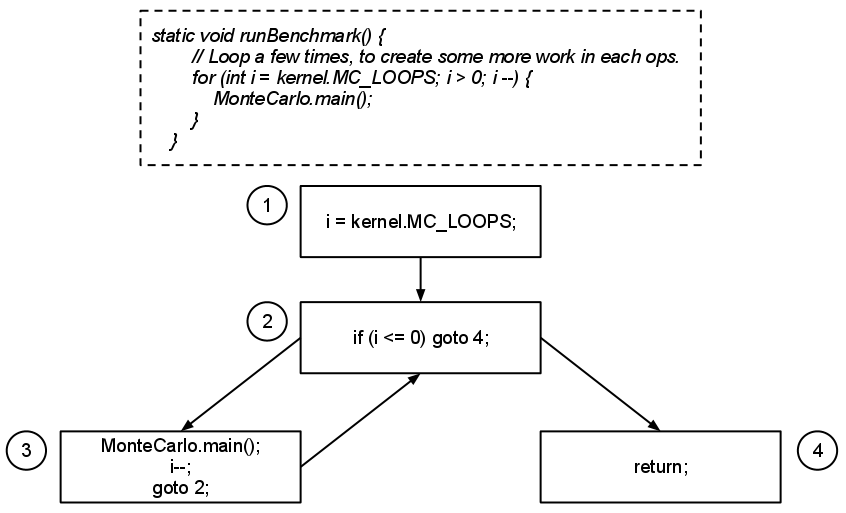
\includegraphics[width=8cm]{imgs/cfg.png}
\caption{An example of a control flow graph for a the \textit{rubBenchmark} method of \textit{SciMark} benchmark from the \textit{SPECjvm2008} benchmarks
\cite{specjvm2008}.}
\label{fig:cfg}
\end{figure}

In this project, we plan to use static execution path information (e.g. number of if statements, fields written to) to construct a Bayesian network that is
capable of predicting the probability that a given path is hot. We adopt the same approach suggested by Buse and Weimer \cite{buse2009road} to classify
execution paths after applying two main modifications to it. First, we statically enumerate execution paths based on the control flow graph of each method
individually rather than the control flow graph of each individual class. We adjust the feature description model of the execution path accordingly. We then
cluster the statically enumerated paths using a simple k-means clusterer into two clusters (hot and cold). The results from the clusterer are used as the ground
truth. Afterwards, we train a Bayesian network using one training dataset, and test four different test datasets against it. Second, we evaluate our model using
the more recent SPECjvm2008 \cite{specjvm2008} benchmarks as opposed to the obsolete SPECjvm98 \cite{specjvm98} benchmarks.

The rest of the report is structured as follows. We discuss related work in Section \ref{sec:bg}. In Section \ref{sec:implementation}, we provide an in depth
discussion for the implementation details of our model. We then provide our the experimental results of our model in Section \ref{sec:results} followed by
discussion and some proposed future work in Section \ref{sec:difficulties}. Finally, we conclude the report in Section \ref{sec:conc}.

\section{Related Work}
\label{sec:bg}
Static branch prediction is the closest work to the idea presented in this project. The purpose of static branch prediction is to statically classify branch
edges in a given execution path as \textit{taken}, or \textit{not-taken} according to some criteria. Information about branch edges can be gathered from
workloads (profile-based branch prediction) or inferred statically from the control flow graph information (program-based branch prediction).

Ball and Larus \cite{ball1993branch} present a program-based branch predictor that performs well for a large and diverse set of programs written in C and
Fortran. The core of their model is based on simple heuristics for predicting non-loop branches, which dominate the dynamic branch count of many programs.
A more recent study shows that those heuristics achieve an average of 70\% prediction rate with 33\% miss rate \cite{calder1997evidence}. The same study
further extends those heuristics by using a richer static feature set and employing neural network learning techniques. The authors were able to decrease
the miss rate to an average of 21\% but this came at the cost of decreasing the prediction rate to an average of 50\%.

Focusing only on branch edge information is not useful for hot path identification. Analyzing the whole execution path provides a richer set of information
than individual branch edge information \cite{buse2009road}. Thus, it is more useful to design a path-based formal model for prediction. This is the option we
opted for in this project.

Our work is inspired by the work of Buse and Weimer \cite{buse2009road} where they present a technique for statically estimating the runtime frequency of
program paths. The results of such technique can be used to support or improve many types of static program analyses. The authors report an accuracy of 90\%
for their model. However, they do not report on their miss rates. Moreover, they do not provide any details as to how they built the Bayesian network used for
prediction or the precision and the recall values recorded for each experiment. In addition, the authors use workloads automatically generated from the
SPECjvm98 benchmarks \cite{specjvm98} to get the ground truth for path execution frequency to train and evaluate their model. This defies one of their major
goals, attempting to model indicative execution frequency by avoiding the usage of automatically generated workloads. In this work, we only depend on
information gathered from statically enumerated execution paths and do not make use of automatically generated workloads.

\section{Model Construction}
\label{sec:implementation}
In any given imperative programming language (e.g Java), each method can be represented as a control flow graph (cfg). This cfg defines all possible execution
paths among which only one will be followed in a given execution scenario. The goal of this work is to describe a feature model for a given static execution
path (hereafter, path). Based on that model, the path can be classified as either a hot path or a cold path. Our approach consists of four major steps: path
description, path enumeration, dataset generation, and finally the construction of the Bayesian network used for testing. The current implementation of our
approach supports Java, but the model still applies to other imperative languages.

\subsection{Path Description Model}
As mentioned earlier, we adopt a similar path description model to the one proposed by Buse and Weimer \cite{buse2009road}. However, we apply some modifications
to the path description model to comply with our definition of a path. We define a path as an execution path for a given method that can be statically
enumerated from the control flow graph of that method. Consequently, we do not take into consideration features like \textit{this} and \textit{return
statements} from their model \cite{buse2009road} because these features do not reveal more information in the context of a method. Any given method has a
\textit{this} parameter and a \textit{return statement}. Table \ref{tab:features} provides a full list of the features that are used to describe a path. A
path is eventually represented by a vector of the counts of those features. Since we assume that hot paths induce minimal change in program state, the lower the
values of the feature vector, the more probable it is that the path is hot.

\begin{table}[h!]
\centering
\begin{tabular}{|c|c|}
\hline
\textbf{Feature} & \textbf{Description}\\
\hline\hline
== & equal condition \\
\hline
new & any new expression \\
\hline
= & assignment statements \\
\hline
. & pointer dereferences \\
\hline
fields & class fields usage  \\
\hline
fields written & class fields written to \\
\hline
invocations & all method invocations \\
\hline
goto & goto statements \\
\hline
if & if statements \\
\hline
locals & local variables usage \\
\hline
statements & total number of statements \\
\hline
throws & throw statements \\
\hline
\end{tabular}
\centering
\caption{The set of features defining a path description model.}
\label{tab:features}
\end{table}

\subsection{Path Enumeration}
We use the Soot \cite{vallee1999soot} APIs to analyze the input source code, and generate the control flow graphs for each method from the input classes. For a
given method, we generate its control flow graph, then apply a modified version of the depth-first search algorithm to the graph to enumerate potential paths.
Algorithms \ref{alg:process} and \ref{alg:search} show a pseudo-code for the algorithm used to enumerate the paths for a given control flow graph, and paths
starting at a given block in the graph respectively. We assume that a path through a loop construct represents all paths that take the loop once or more. This
prevents the generation of an unbounded number of potential paths. Each path is represented as a stack of basic blocks, where each basic block is sequence of
source code statements.

\begin{algorithm}[h!]
\caption{Enumerate potential paths for a given CFG}
\label{alg:process}
\textbf{Input:} {cfg for a method} \\
\textbf{Output:} {potential execution paths} \\ \\
\textbf{process}(cfg) \{
\begin{algorithmic}
\STATE Initialize $potentialPaths$ = \{\}
    \FOR{$head$ in $cfg.getHeads()$}
     \STATE Initialize $path$ = \{\}
     \STATE Initialize $headPaths$ = \{\}
     \STATE $search(head, path, headPaths)$
     \STATE $potentialPaths.addAll(headPaths)$
    \ENDFOR
\end{algorithmic}
\}
\end{algorithm}

\begin{algorithm}[h!]
\caption{Search for paths starting at a given CFG block}
\label{alg:search}
\textbf{Input:} {current block, current path, and the result so far} \\
\textbf{Output:} {potential paths starting at a given CFG block} \\ \\
\textbf{search}(block, path, result) \{
\begin{algorithmic}
   \IF{\textit{stuck in a cycle}}
    \STATE $return$
   \ENDIF
   \STATE $path.push(block)$ \COMMENT {path is a stack of blocks}
   \IF{\textit{block is a tail}}
    \STATE $result.add(path)$
    \STATE $path.pop()$ \COMMENT {to get other paths}
    \STATE $return$
   \ENDIF
   \FOR{$successor$ in $block.getSuccessors()$}
    \STATE $search(successor, path, result)$
   \ENDFOR
   \STATE $path.pop()$ \COMMENT {no path found}
\end{algorithmic}
\}
\end{algorithm}

Once all potential execution paths are generated, we analyze each one to compute its feature vector (i.e. the vector of count of each feature for this path).
This task is performed by our feature extraction tool that takes a given execution path and uses the Soot \cite{vallee1999soot} APIs to extract those features.
The feature vector of the path gets updated accordingly. Finally, we store the generated feature vectors in a format that can be recognized by the data mining
software we are using, WEKA \cite{hall2009weka}. We chose to store the feature vectors in ARFF format, an ASCII text file that describes a list of instances
sharing a set of attributes \cite{arff}.

\subsection{Dataset Generation}
\label{dataset-generation}
Generating an indicative dataset of execution paths is not an easy task. One has to develop (or gather) real life applications and analyze them to compile such
a dataset. SPECjvm2008 \cite{specjvm2008}, fortunately, already provides a benchmark suite for measuring the performance of a Java Runtime Environment (JRE),
containing several real life applications and benchmarks (e.g. derby, javac, crypto, xml) focusing on core Java functionality. This dataset was compiled
to be used instead of the obsolete SPECjvm98 \cite{specjvm98} used in \cite{buse2009road}.

As with any learning algorithm, we had to divide our dataset into a training set, and a test set. We limit our training set to all paths generated from control
flow graphs that have at most 10 nodes (i.e. basic blocks). On the other hand, we generate four test sets each consists of all paths generated from
control flow graphs that have, 10-20, 20-30, 30-40, and 40-50 nodes respectively. We could not go beyond that number of nodes per control flow graph due to the
limited RAM we have on our machine (1 GB). This was also another reason why we had to split the dataset into 5 subsets, one used as a training dataset, and the
others as test datasets.

\begin{table}[h!]
\centering
\resizebox{0.5\textwidth}{!}{
\begin{tabular}{|c|c|c|c|}
\hline
\textbf{CFG Node Count} & \textbf{No. of Instances} & \textbf{Runtime (msecs)} & \textbf{Codename} \\
\hline\hline
1 - 10 & 2087 & 619 & Training \\
\hline
11 - 20 & 2667 & 1130 & Test-20 \\
\hline
21 - 30 & 6730 & 2342 & Test-30 \\
\hline
31 - 40 & 71772 & 47461 & Test-40 \\
\hline
41 - 50 & 143078 & 92895 & Test-50 \\
\hline
\end{tabular}}
\centering
\caption{The characteristics of the datasets with the class attribute missing.}
\label{tab:no-class}
\end{table}

Since WEKA \cite{hall2009weka} has to know the ground truth about both the training set and the test sets, we first generate all the datasets with their class
attribute missing (Table \ref{tab:no-class}). We then feed each of our 5 datasets to WEKA as a training set and apply simple k-means clustering algorithm to
them, ignoring the missing class attribute. The output of each run results in two clusters per dataset, each cluster has an average count per feature (centroid
of the cluster). The cluster with the smaller centroid values is considered to be the hot paths cluster, the other one is the cold paths cluster (based on our
assumption in Section \ref{sec:intro}). Table \ref{tab:avg} summarizes the feature counts of the cluster centroid for what we identified as the hot paths
cluster for each dataset.

\begin{table*}[t!]
\centering
\begin{tabular}{|c|c|c|c|c|c|}
\hline
\textbf{CFG Node Count} & \textbf{1 - 10} & \textbf{11 - 20} & \textbf{21 - 30} & \textbf{31 - 40} & \textbf{41 - 50} \\
\hline\hline
ASSIGNMENTS & 3.714 & 16.9907 & 23.1365 & 69.3282 & 56.5917 \\
\hline
DEREFERNCES & 2.9033 & 4.0865 & 6.5968 & 12.4859 & 13.8164 \\
\hline
EQUAL & 0.142 & 1.9292 & 2.5739 & 5.554 & 13.8748 \\
\hline
FIELDS & 1.1788 & 2.0805 & 4.2011 & 9.7243 & 10.5063 \\
\hline
FIELDS\_WRITTEN & 0.4753 & 0.2735 & 0.6598 & 0.7413 & 2.4874 \\
\hline
GOTO & 0.5498 & 7.7237 & 8.4264 & 13.8151 & 23.5838 \\
\hline
IF & 0.4308 & 6.5747 & 7.0163 & 10.756 & 19.88 \\
\hline
INVOCATIONS & 2.3236 & 12.4984 & 16.3752 & 74.8947 & 40.7381 \\
\hline
LOCALS & 10.4997 & 45.1786 & 58.4237 & 194.84 & 132.9246 \\
\hline
NEW & 0.4252 & 0.8422 & 1.7663 & 8.1021 & 2.6921 \\
\hline
STATEMENTS & 7.9081 & 30.7885 & 38.9947 & 120.8035 & 88.2042 \\
\hline
THROWS & 0.0334 & 0.025 & 0.0556 & 0.0238 & 0.0088 \\
\hline\hline
\textbf{No. of Iterations}  & 13 & 20 & 5 & 9 & 9 \\
\hline
\end{tabular}
\centering
\caption{Hot paths clusters centroids.}
\label{tab:avg}
\end{table*}

The feature counts of the centroid of each dataset provide us with an average threshold for the feature counts for hot paths in that dataset. Therefore, we
have to properly classify the paths as hot or cold in each dataset based on the respective centroid values. Therefore, we had to go back to our
previously generated datasets, and label each path accordingly. We consider the resulting class as the ground truth that will be used afterwards to evaluate
our model. The pseudo-code for our path classification algorithm is shown in Algorithm \ref{alg:classify}. To classify a path, we loop over all the
feature counts of the given path. If the count of a feature is greater than the average count of the feature for the corresponding cluster centroid. We then
increment the probability that this path is not hot by $\frac{1}{number of features}$. Finally, the path is a hot path if this probability is less than or equal
to 0.5, it is cold otherwise.

\begin{algorithm}[h!]
\caption{Classify a given execution path}
\label{alg:classify}
\textbf{Input:} {path, and cluster centroid feature vector} \\
\textbf{Output:} {class (hot, or cold)} \\ \\
\textbf{label}(path, centroid) \{
\begin{algorithmic}
   \STATE Initialize $probability$ = 0
   \FOR{$feature$ in $path.getFeatures()$}
    \IF{path.feature.count() $\geq$ centroid.feature.count()}
     \STATE $probability$ += 1 / \textit{no. of features}
    \ENDIF
   \ENDFOR
   \IF{probability $\leq$ 0.5}
    \STATE \textit{return hot}
   \ELSE
    \STATE \textit{return cold}
   \ENDIF
\end{algorithmic}
\}
\end{algorithm}

\subsection{Bayesian Network Construction}
We use WEKA to build our Bayesian network based on the training set only (i.e. paths from control flow graphs with at most 10 nodes). The network is built
using K2 (a greedy Bayesian network construction algorithm) with maximum number of parent nodes = 5 and a simple estimator with prior probability = 0.5. The
average time taken to build our Bayesian network is 0.22 seconds. Due to the settings of WEKA, the Bayesian network has to be rebuilt each time a new test set
is supplied. Figure \ref{fig:bayes} shows our Bayesian network using Training as the training dataset and Test-20 as the test dataset.

\begin{figure*}[t!]
\centering
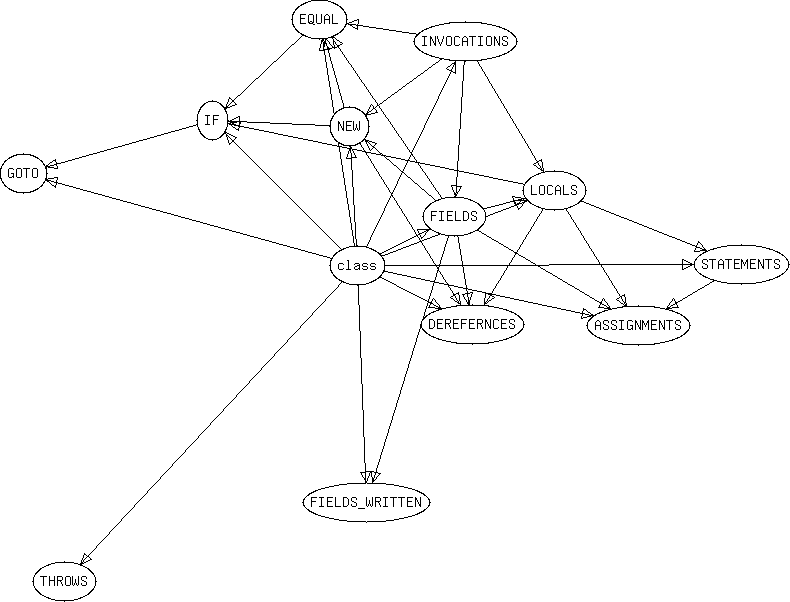
\includegraphics[width=\textwidth]{imgs/bayes.png}
\caption{Bayesian network using Training dataset, and Test-20 test dataset.}
\label{fig:bayes}
\end{figure*}

\section{Model Evaluation}
\label{sec:results}
We performed 4 experiments to evaluate the predictive power of our model. In each experiment, we used the same training dataset (Training) and a different test
dataset. All experiments model our problem as a classification problem, i.e. label each path as \textit{hot} or \textit{cold}.

\subsection{Experimental Setup}
As mentioned earlier, we used the Soot \cite{vallee1999soot} APIs to implement the algorithms described in Section \ref{sec:implementation}, and WEKA
\cite{hall2009weka} APIs and Explorer GUI for machine learning. We ran all our experiments on an HP laptop with Intel Centrino Duo 2.0 processor, 1GB RAM,
running Ubuntu 10.10 (Maverick) with 2.6.3.23 kernel version.

\subsection{Results}
We evaluated our model based on 4 parameters:
\begin{itemize}
  \item true positive rate: correctly classified paths (compared to our ground truth),
  \item false positive rate: misclassified paths (compared to our ground truth),
  \item precision: the fraction of correct instances among those that the algorithm classifies as hot paths (i.e. a measure of exactness or fidelity), and
  \item recall: the fraction of correct instances among all instances that are actually hot (i.e. a measure of completeness).
\end{itemize}

Figure \ref{fig:precision} shows a plot for the precision values for the various test datasets. Test-40 yields the best precision value (0.917), while the
lowest precision value achieved by our model (0.829) is obtained using Test-30. On the other hand, Figure \ref{fig:recall} shows a plot for the recall values
for various test datasets. The best recall value (0.909) is achieved using Test-40, while the lowest recall value achieved by our model (0.735) is obtained
using Test-20. Figure \ref{fig:precision-recall} compares the precision and recall values for each test dataset. Table \ref{tab:fmeasure} reports the F-measure
values for each test dataset.

We were very intrigued by the fact that Test-40 achieved the best possible tradeoff between precision and recall (Figure \ref{fig:precision-recall}), and the
highest F-measure (Table \ref{tab:fmeasure}). This observation needs more thorough investigation to be able to arrive at the reasons why this specific test
dataset achieves such high scores. However, our intuition is that for Test-20 and Test-30 the model probably overfits the Training dataset which consists of
only 2087 instances as opposed to 2667 and 6730 instances in the case of Test-20 and Test-30 respectively (Table \ref{tab:no-class}). When we use a test dataset
of much larger number of instances (Test-40 has 71772 instances), the overfitting problem is no longer there due to the big difference between the number of
instances in the training and the test datasets. However, this conclusion requires carrying out more experiments to be validated.

\begin{figure}[h!]
\centering
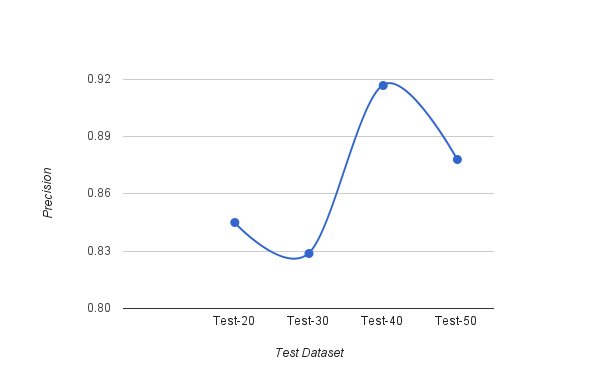
\includegraphics[width=0.5\textwidth]{imgs/precision.png}
\caption{Precision values for the various test datasets.}
\label{fig:precision}
\end{figure}

\begin{figure}[h!]
\centering
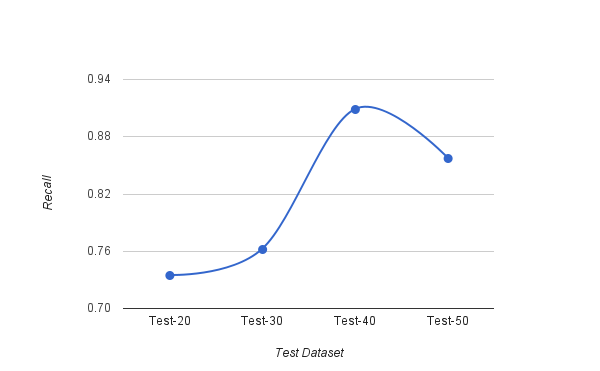
\includegraphics[width=0.5\textwidth]{imgs/recall.png}
\caption{Recall values for the various test datasets.}
\label{fig:recall}
\end{figure}

\begin{figure}[h!]
\centering
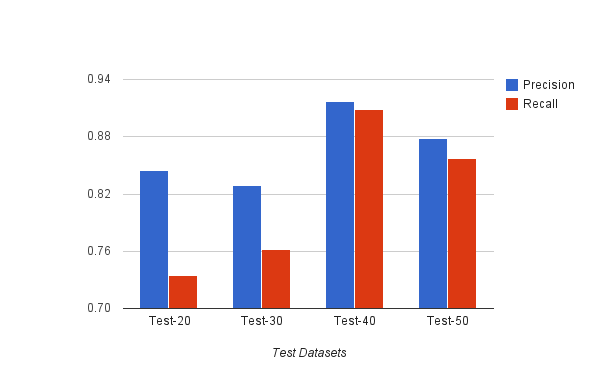
\includegraphics[width=0.5\textwidth]{imgs/precision-recall.png}
\caption{Precision vs Recall values for the various test datasets.}
\label{fig:precision-recall}
\end{figure}

\begin{table}[h!]
\centering
\begin{tabular}{|c|c|}
\hline
\textbf{Test Dataset} & \textbf{F-Measure}\\
\hline\hline
Test-20 & 0.734 \\
\hline
Test-30 & 0.729 \\
\hline
Test-40 & 0.876 \\
\hline
Test-50 & 0.798 \\
\hline
\end{tabular}
\centering
\caption{The F-measure for the various test datasets.}
\label{tab:fmeasure}
\end{table}

\subsection{Threats to Validity}
There are two threats to validity for the experiments we carried out. First, overfitting is inevitable when the sizes of the training data and the test data
are very small and close to each other (e.g. the case of Training and Test-20). However, we tried as much as possible to overcome this challenge by selecting
our datasets to be mutually exclusive of each other. It remains to test our model, using our current training set, against different set of benchmarks to
experimentally prove that the overfitting problem has been resolved. Second, we compare the resulting classification of our model to the ground truth that we
obtain from our clustering process in the dataset generation step (Section \ref{dataset-generation}). This ground truth might not match the real-life ground
truth, i.e. the average counts of hot paths from real program traces. Eliminating this threat to the validity of our model requires carrying out more
experiments with real-life program traces.

\section{Conclusion and Future Work}
\label{sec:conc}
In this project, we used static execution path information (e.g. number of if statements, fields written to) to construct a Bayesian network that is
capable of predicting the probability that a given path is hot. We modified the approach suggested by Buse and Weimer \cite{buse2009road} to classify
execution paths after applying two main modifications to it. First, we enumerate static paths for each individual method. Second, we evaluate our model using
the more recent SPECjvm2008 \cite{specjvm2008} benchmarks as opposed to the obsolete SPECjvm98 \cite{specjvm98} benchmarks. Our experiments have shown that our
model achieves the best precision/recall tradeoff when using Training as the training dataset, and Test-40 as the test dataset. In the worst case (i.e. using
Test-20 as the test dataset), our model achieves a precision of 0.845 and a recall of 0.735. In the future, it would be useful to investigate other benchmarks
to check whether our model suffers from overfitting or not. Finally, we are curious to know the effect of using the ground truth obtained from
real-life program traces as opposed to our clustering technique.

{\small
\bibliographystyle{ieee}
\bibliography{references}
}

\end{document}